\subsection{Polarizers and wave plates}
Date of carrying out experiment: 8th of July, 2019 \\ \\
This first part of the experiment has the purpose of getting used
to the following optical devices: polarizers, beam splitters and waveplates.
The laser used in this part of the experiment has a wavelength of $632.8$
nm and a power output of less than $1$ mW.

\subsubsection{Brewster's angle}
First, we would like to find Brewster's angle. This allows us to
later on calibrate the optical devices. For this, we take a glass plate
and mount it in front of the laser at an angle $\alpha$. This angle can now
be varied. If the angle between the incoming
beam and the surface of the glass plate equals Brewster's 
angle, then the reflected beam contains only photons that are polarized
perpendicular to the plane of incidence. \\ \\ This can in principle
be verified easily by mounting a polarizer in the path of the reflected
beam, but the polarizers are not yet calibrated. This means that we have
to turn the polarizers by $360^\circ$ for each angle $\alpha$. We're
looking for the setup which lets us filter out the maximum amount of light.
A minimum in intensity tells us that the polarizer filters out all or
almost all
of the light, which means the beam contains only a single polarization
component. This is exactly what one would expect at Brewster's angle. \\ \\
Unfortunately, it's not easy to do this in a precise way, since two
quantities have two be varied at the same time: the angle $\alpha$ and
the angle of the polarizer. Also, the laser beam is polarized linearily.
This means, that both the reflected and the refracted/transmitted beam
are polarized. It is always possible to block the reflected ray using a
polarizer. Because of this, we mount a quarter-waveplate between
laser and glass plate to make sure both components are present. \\ \\
Our result:
$$\alpha_{Brewster}\approx(60\pm10)^\circ$$
Now we want to observe what happens when we use other optical devices after
the beam has been reflected at Brewster's angle. As expected, the beam
splitter splits the beam into one beam with very high intensity and
another beam whose intensity is almost zero. \\
A polarizer either blocks the beam or has no effect,
depending on orientation.

\subsubsection{Second glass plate}
A second glass plate is mounted perpendicular to the plane of incidence of
the first glass plate, so that the beam reflected on the first glass plate
is reflected off of it. The incoming beam is once again split into two.
In contrast to the previous observation, it is now possible to use a
polarizer to block both beams for any orientation of the glass plate.
This is to be expected, since the beam that was reflected on plate 1 is
polarized, so both beams after plate 2 are polarized as well.

\newpage
\subsubsection{Polarizers}
Now we want to calibrate the polarizers, i.e. we want to know for which
angles linearily polarized light is blocked. For this, we use a similar
setup as in the last observation. The laser is reflected off the glass
plate at Brewster's angle through the polarizer. By varying the orientation
of the polarizer and looking for a minimum of the intensity, we find: \\ \\
blocking angle for polarizer 130000: $\alpha_1=(100 \pm 5)^\circ$ \\
blocking angle for polarizer 130200: $\alpha_2=(101 \pm 5)^\circ$ \\ \\
Because we know that the beam reflected from the glass plate is polarized
vertically, we can conclude that the polarizers are calibrated in
such a way that the vertically polarized laser light can pass through the
polarizer if it is set to $\approx10^\circ$,

\subsubsection{Beam splitters}
We want to find out the polarization of the two beams exiting a beam
splitter. After mounting a polarizer behind the beam splitter and looking
for which angles the beams can pass through, we observe that both beams
show maximum intensity for an angle of $0^\circ$ and minimum for $90^\circ$.

\subsubsection{Half-waveplates}
Now we'd like to observe how a half-waveplate or a quarter-waveplate
influences the polarization state of the light beam. \\ \\
First, we take a look at the half-waveplate. It is mounted between the
glass plate and a polarizer. Minima are observed for a the angles
$2^\circ$, $91^\circ$, $182^\circ$ and $270^\circ$ with uncertainties of
about $5^\circ$. These are the positions where the incident polarization
is rotated by $90^\circ$.

\subsubsection{Quarter-waveplates}
Herfore, a quarter-waveplate is mounted between two polarizers.
For waveplate a, the minima are observed at the angles $8^\circ$,
$98^\circ$, $188^\circ$ and $279^\circ$. For waveplate b,
the minima are observed for the angles, $59^\circ$,
$151^\circ$, $241^\circ$ and $330^\circ$ with an uncertainty of
about $5^\circ$

\subsubsection{Setup from fig. \ref{wave_plate_setup}}
Next, we realize the experimental setup shown in figure
\ref{wave_plate_setup1}. Waveplate a is set to the angle
$8^\circ+45^\circ=53^\circ$ and waveplate b to $59^\circ+45^\circ=104^\circ$
We find minima for the polarizer angles $180^\circ$ and $360^\circ$.
If the second waveplate is turned by $180^\circ$ around the axis on
which it is mounted, we get minima at $88^\circ$ and $266^\circ$. \\ \\
To realize the setup from figure \ref{wave_plate_setup2}, we need to
rotate the initial polarization by $45^\circ$. This can be done with a
half-waveplate that is set to an angle that corresponds to halfway from
a minimum to the next maximum. That is about $22.5^\circ$.
The waveplate angle for a is now $59^\circ$, the angle for b is $8^\circ$.
The minima are at angles of $25^\circ$ and $205^\circ$.
After turning waveplate b on its axis, the minima are at roughly the same
positions as before. This is two be expected, \textcolor{red}{because...}
\begin{figure}[h!]
    \centering
    \begin{subfigure}{.5\textwidth}
        \centering
        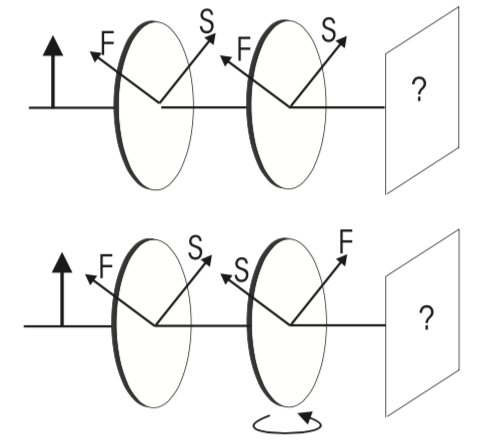
\includegraphics[width=.8\linewidth]{wave_plate_setup1}
        \caption{waveplate setup 1}
        \label{wave_plate_setup1}
    \end{subfigure}%
    \begin{subfigure}{.5\textwidth}
        \centering
        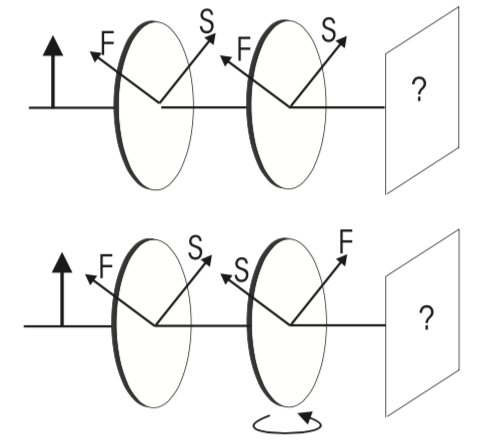
\includegraphics[width=.8\linewidth]{wave_plate_setup2}
        \caption{waveplate setup 2}
        \label{wave_plate_setup2}
    \end{subfigure}
    \caption{setups for waveplate experiment}
    \label{wave_plate_setup}
\end{figure}

\newpage
\subsubsection{Mirror between quarter-waveplates}
Now, a mirror is positioned between the two quarter-waveplates
in a way so that the angle of reflection is bigger than $45^\circ$
(total angle bigger than $90^\circ$). After this is done, we do not
not observe any dependance of the intensity on the polarizer angle.
We conclude that the light is circularily polarized.
\textcolor{red}{maybe both quarter-waveplates were switched, wrong angles}

\subsubsection{Reflection back into quarter-waveplate}
The laser beam is lead through a quarter-waveplate and onto a mirror.
The mirror is positioned perpendicular to the optical axis, so that
the beam goes back through the quarter-waveplate. \\
%During reflection, the beam undergoes a phase shift by half a wavelength,
%so that 
If the quarter-waveplate is set to an angle of $8^\circ$, 
the mimima are found for the polarizer angles $165^\circ$ and $350^\circ$.
If it is instead set to $53^\circ$, the minima are at $85^\circ$ and
$265^\circ$

\subsubsection{Reflection back into half-waveplate}
The same as above is done again, this time with a half-waveplate.
At a waveplate angle of $2^\circ$, no minima could be found.
Then we set the waveplate angle to $47^\circ$. Here, we did find minima
at $75^\circ$ and $255^\circ$.

\subsubsection{Mirror}
A mirror is set up in a way such that the laser beam is reflected from
the glass onto the mirror in an angle bigger than $45^\circ$.
Minima are detected for the polarizer angles of $90^\circ$ and $270^\circ$.
Now we do the same for perpendicular polarization. Now the minima are
at $186^\circ$ and $6^\circ$.

\subsubsection{Lamp light through optical isolator}
Looking through the optical isolator at the ceiling lamp, the lamp
appears either orange or green, depending on the orientation of the
isolator. \textcolor{red}{Why?}

\subsection{Electro-optical effect}
Date of carrying out experiment: 9th of July, 2019 \\ \\
The laser used in this part of the experiment produces light with a
wavelength of $\lambda=635$ nm and outputs a power of less than $1$ mW.
The material in the Pockels cell is  LiNbO$_3$,
which is a uniaxial crystal with $3m$-symmetry ($n_1=n_2=n_o, n_3=n_e$) \\
\textcolor{red}{Pockels coefficients are very hard to measure,
can be affected by crystal impurities}
%In the first part of this experiment, the change of the index of
%refraction will be measured directly. In the second part, the
%effect will be observed by measuring the polarization state of light 
%before and after traversing the crystal.

\subsubsection{Measurement of amplification}
First, we want to determine the amplification factor of the
high voltage power supply. The DC power supply is connected to the
amplifier. For several DC voltages $U_0$ we record the corresponding
high voltage value $U_{amp}$.
\begin{center}
    \begin{tabular}{l|c|c|c|c|c|c|c|c|c|c|c|c|c}
        $U_0$ [V] & 6.50 & 6.00 & 5.50 & 5.00 & 4.50 & 4.00 &
                  3.50 & 3.00 & 2.50 & 2.00 & 1.50 & 1.00 & 0.50 \\
        \hline
        $U_{amp}$ [kV] & 1.95 & 1.80 & 1.65 & 1.50 & 1.35 & 1.20
                       & 1.05 & 0.90 & 0.75 & 0.60 & 0.45 & 0.30 & 0.15
    \end{tabular}
\end{center}
We take care not to let the amplified
voltage get higher than $2.00$ kV, this is the maximum voltage the
Pockels cell can endure. The uncertainty on the display of the power
supply devices is $0.005$ V for $U_0$ and $0.005$ kV for $U_{amp}$.
\textcolor{red}{other error?}

\subsubsection{Calibration of Pockels cell}
To determine the directions of the optical axes in the Pockels cell,
it is placed between two polarizers. The polarizers are oriented
perpendicular to each other, so that without the cell no light can pass
through.
\begin{center}
    \begin{tabular}{c|c}
        polarizer serial number & polarizer angle \\
        \hline
        130000 & $100^\circ$ \\
        130200 & $10^\circ$
    \end{tabular}
\end{center}
The laser light passes first through the polarizer 130200, then through
the Pockels cell and 130000. \\ \\
The Pockels cell angle scale goes from $-90^\circ$ to $+90^\circ$ and
the minima are observed for the Pockel cell angles $10^\circ$ and
$-80^\circ$. Minima are observed when the laser beam is parallel to
either the fast or the slow axis of the crystal.

\subsubsection{Mach-Zehnder interferometer}
We would like to quantify the effect that the Pockels cell has on the phase
of a laser beam. For this, a Mach-Zehnder interferometer is set up.
The setup can be seen in figure \ref{mach_zehnder_interferometer}. \newpage
\begin{figure}[h!]
    \center
    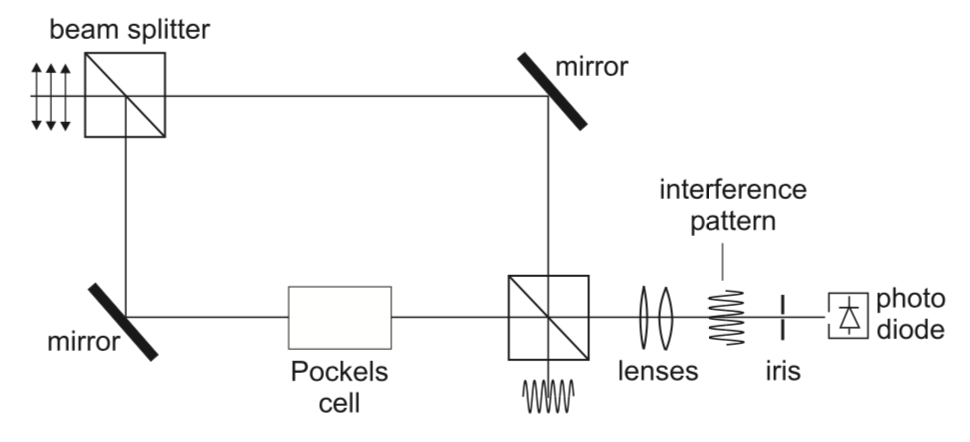
\includegraphics[width=.75\textwidth]{mach_zehnder_interferometer}
    \caption{setup of Mach-Zehnder interferometer}
    \label{mach_zehnder_interferometer}
\end{figure} \noindent
After the separated laser beams are joined back together, we want to make
sure they are as close to being parallel as possible. A piece of paper
is held into the beam directly behind the beam splitter. The mirrors
are oriented in such a way that both beams hit the paper in a single spot.
Then the distance between the piece of paper and the beam splitter is
increased and the mirror positions once again adjusted. \\ \\
A triangular waveform is chosen on the function generator. The frequency
of this signal is $\approx 3.5$ Hz \textcolor{red}{!!!}. The generator
is connected to the amplifier, the amplifier to the Pockels cell.
The output of the function generator as well as the photo diode are
connected to the oscilloscope. The oscilloscope output can be saved to
.csv and used for later analysis. \\ This is done for the Pockels cell
angles $-80^\circ$, $10^\circ$, $-90^\circ$ and $90^\circ$

\newpage
\subsubsection{Manipulation of polarization and intensity}
The setup is shown in figure
\ref{manipulation_of_polarization_and_intensity}. The angle between
the polarization axes of the filters and the Pockels cell need to be
$45^\circ$, \textcolor{red}{because...} \\ \\
The angle of the first filter (set to vertical polarization) is
$10^\circ$, the second one $100^\circ$. For the Pockels cell, we know from
the calibration that an angle of $+45^\circ$/$-45^\circ$ relative to the 
vertical polarization axis corresponds to an actual angle setting of
$55^\circ$/$-35^\circ$ at the Pockels cell. \\ \\
The transmitted power on the photodiode is recorded as a function of
the applied high voltage by choosing again a triangular waveform on the
the function generator. This is done for the angles $-45^\circ$ and
$45^\circ$.
\begin{figure}[h!]
    \center
    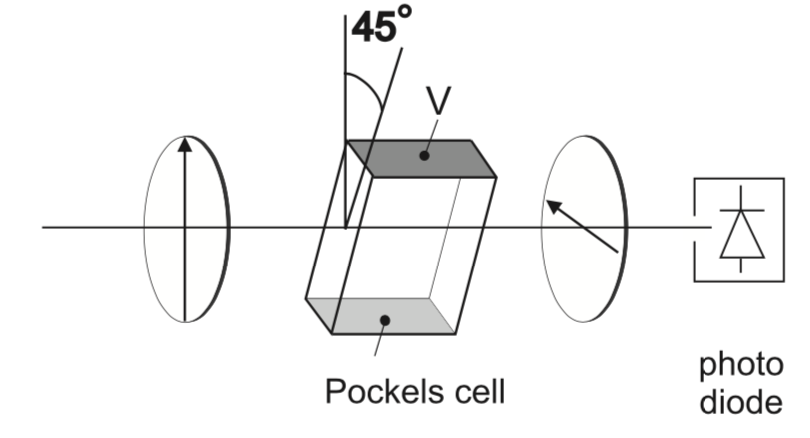
\includegraphics[width=.5\textwidth]{manipulation_of_polarization_and_intensity}
    \caption{manipulation of polarization and intensity}
    \label{manipulation_of_polarization_and_intensity}
\end{figure}

\subsubsection{Linear amplitude modulation}
Now, the Pockels cell is connected to a DC high voltage.
The amplifier is set to intern. Multiple
measurements will be made, the DC voltage will be varied from one
measurement to the next. A modulated signal is added to the DC voltage
and the resulting signal is given to the Pockels cell.
The frequency of the modulated (sinoid) signal is about $1.0000\pm0.0005$ kV.
\\ \\ For the following DC voltages and Pockels cell angles the waveform
is saved:
\begin{center}
    \begin{tabular}{l|cccc}
        Pockels cell angle & $-35^\circ$ & $55^\circ$
                           & $-90^\circ$ & $90^\circ$ \\
        \hline
        DC voltage & 0.60 kV & 0.46 kV & 0.49 kV & 0.45 kV
    \end{tabular}
\end{center}
%For our setup the half-wave voltage is given as $V_\pi=380$ V
%in the lab course script\cite{F85}. Our first measurement is done at a
%voltage of $330$ V, then we increase the voltage in steps of $10$ V
%until we reach $430$ V.


\begin{comment}
\newpage
\subsubsection{Phase shift due to electro-optical modulation}
\begin{enumerate}
    \item $\vec E$-field along optical axis
    \item laser beam is incident perpendicular to the field
    \item HV supply: output should be between $0$ V and $1.8$ kV
    \item measure amplification factor of HV amplifier
    \item evaluate measurements
\end{enumerate}

\subsubsection{Mach-Zehnder interferometer}
To quantify the extent by which the phase is shifted, we use a
Mach-Zehnder interferometer.
\begin{enumerate}
    \item why non-polarizing beam splitters
    \item direction of optical axes
    \item good overlap of arms
    \item setup measurement
    \item output intensity as function of applied voltage (for both axes)
    \item compare results
    \item just for fun: speaker
\end{enumerate}

\subsubsection{Manipulation of polarization and intensity}
\begin{enumerate}
    \item why Pockels cell at $45^\circ$
    \item measure transmitted power as function of HV for $\pm45^\circ$
\end{enumerate}

\subsubsection{Linear amplitude modulation}
0.6 -35, 0.46 55
0.49 -90, 0.45 90
\begin{enumerate}
    \item ...
\end{enumerate}
\end{comment}


\newpage
\subsection{Acousto-optical effect}
Date of carrying out experiment: 10th of July, 2019

\subsubsection{Experiments with a single AOM}
A high frequency acoustic signal is applied to the crystal by connecting
a DC voltage to the VCO. \\ \\
A fairly symmetric interference pattern showing 5 maxima can be realized
with the frequency-controlling voltage being set to
$9.4$ V and the VCO level-controlling voltage to $1.9$ V. \\ \\
For different values of the VCO frequency-controlling voltage $U_f$,
we record the distance $a_i$ between the maxima of order $0$ and $i$.
The AOM frequency can be calculated from the applied voltage. Since the
range if the AOM is $(110\pm25)$ MHz\cite{F85} and the voltage can be
varied by $\pm10$ V, we conclude that varying the voltage by $1$ V
corresponds to a frequency change of $2.5$ Hz. \\ \\
The distance between the crystal and the screen is $d=(194\pm3)$. \\
\begin{center}
    \begin{tabular}{l|cccccccccc}
        $U_f$ [V] & 1 & 2 & 3 & 4 & 5 &
        6 & 7 & 8 & 9 & 10 \\
        \hline
        $a_1$ [cm] & 4.4 & 4.3 & 4.1 & 3.9 &
        3.7 & 3.5 & 3.2 & 3.1 & 2.9 & 2.7 \\
        $a_2$ [cm] & - & - & - & 7.8 & 7.4 & 7.1 & 6.6 & 6.4 & 5.9 & 5.6
    \end{tabular}
\end{center} \null \ \\
The uncertainties of the positions
are estimated to be about $2$ mm, since the points
in the interference pattern have a certain spatial extension. \\ \\
Now, we want to compare the intensity of the 0th order maximum with the
intensity of the 1st order maximum. For that, we mount a photodiode in
the path of the laser beam. The photodiode voltage for the undiffracted beam 
is read from the oscilloscope as $U_{0,1}=(96\pm2)$ mV if the diode is
placed directly behind the laser or $U_{0,2}=89\pm2$ mV if the
diode is placed at a certain distance from the cell ($\approx 90$ cm).
The distance between the cell and the laser is $\approx 20$ cm. \\
\begin{center}
    \begin{tabular}{l|cccccccccc}
        $U_f$ [V] & 1 & 2 & 3 & 4 & 5 & 6 & 7 & 8 & 9 & 10 \\
        \hline
        %$U_{max,0}$ [mV] & 88 & 85 & 84 & 86 &
        %85 & $86\pm3$ & 86 & 86 & 85\\
        %$U_{max,1}$ [mV] & 11 & 16 & 14 & 19 &
        %32 & 27 & 25 & $27\pm2$
        $U_{max,1}$ & 46 & 49 & $43\pm2$ & 49 & 77 & $77\pm2$ & 77 & 70 &
        $55\pm2$ & 63
    \end{tabular}
\end{center} \null \ \\
The uncertainties for the voltages are $\pm1$ mV each, if not otherwise
specified. \\
\textcolor{red}{für große $U_f$: Fehler: Maxima werden Striche statt Punkte, nicht alles auf Diode} \\ \\
Because another group was in the room during the measurement, we couldn't
turn off the lights. Because of this, a background measurement is done at
the end. The photodiode voltage with the lights off is
is $100\pm1$ mV. \newpage \noindent
Now, we want to do a similar measurement, but this time vary the amplitude
$A$ instead of the frequency $f$ of the sound wave. This we do by varying the
voltage $U_A$ for the VCO level. The voltage controlling the frequency
is set to $U_f=(7.00\pm0.05)$ V.
\begin{center}
    \begin{tabular}{l|cccccccccc}
        $U_A$ [V] & 0.20 & 0.40 & 0.60 & 0.80 & 1.00 &
        1.20 & 1.40 & 1.60 & 1.80 & 2.00 \\
        \hline
        $U_{max,1}$ & - & $19\pm2$ & $34\pm2$ & $69\pm2$ & 79 & 83 & 82 &
        81 & 83 & 85
    \end{tabular}
\end{center} \null \ \\
The uncertainty of the voltage $U_A$ is estimated to be about $0.05$ V and
stems from the reading process on the display, which can only show
one digit after the comma. As before, the uncertainty of $U_A$
is $\pm1$ if not otherwise specified. \\ \\
\textcolor{red}{nicht symmetrisch ausgerichtet: Problem?}

\subsubsection{Experiments with two  perpendicular AOMs}
For the next experiment, both AOMs are placed near each other
($\approx 1$ cm) and perpendicular to each other. Each of them is 
connected over the amplifier to one of the outputs of the function generator
with two outputs. The setup can be seen in figure \ref{setup_2aom}.
We expect to now see a two-dimensional interference pattern, which
is also what we see. \\ \\ If the offset voltages are increased, the fringes
in the pattern move closer to each other in the corresponding direction
(left/right or up/down depending in which AOM is controlled). \\ \\
When we modulate the sound amplitudes, we see that the interference pattern
starts blinking. This is to be expected, since the amplitude of the
sound wave determines how much the light is refracted in the crystal.
If the amplitude becomes very low, only the unrefracted beam is visible.
The velocity with which the interference pattern moves depends on the
derivative of the modulation function. For example, a triangle function
leads to linear expansion/contraction, while the non-differentiable
block function leads to sudden jumps in the positions of the fringes.
\\ \\ Now we observe the effect on the interference pattern if we
change the phase difference. For a phase difference of $0^\circ$ both
patterns contract/expand at the same times. For $180^\circ$, they move
exactly opposite to one another. For $90^\circ$, the maximum velocity of one
pattern is reached when the other pattern is momentarily at rest. \\ \\
A circle can be drawn at fringe (1, 1),
if the phase difference between the AOMs is
exactly $90^\circ$ and they both have the same amplitude. To draw an
ellipse, both AOMs can be given different amplitudes. If one wants to
draw a circle with e.g. (1, 2), the ampltitudes have to be adjusted
accordingly by the same factor. \\ \\
\textcolor{red}{relation to polarization} \\
The phase shifting box has a similar effect to that of a waveplate,
since the phase of one wave is shifted relative to another. \\ \\
\textcolor{red}{If one frequency is an exact multiple of the other,
Lissajous figures can be created, for example an eight figure for 2:1.
If the ratio between the frequencies is not a natural number,
then the Lissajous figure is not closed, but open.
If the ratio between the frequencies is not a natural number,
then the Lissajous figure is not closed, but open} \\ \\
Now we again want to draw a circle. \\ \\
The difference between a laser and light from e.g. a light bulb is that
the light from the bulb is not linearily polarized, doesn't have a
uniform frequency and is not coherent, i.e. doesn't have the same phase
for all photons. An ideal laser would have these properties.
\textcolor{red}{coherence length/time?}
